%Input preamble
\input{preambleappendix}
%Other parameters
\newcommand{\noutcomes}{95}
\newcommand{\treatsubsabc}{$75\%$}
\newcommand{\treatsubscarec}{$74\%$}
\newcommand{\treatsubscaref}{$63\%$}

%Counts
%Males
\newcommand{\positivem}{$79\%$}
\newcommand{\positivesm}{$37\%$}

%Females
\newcommand{\positivef}{$73\%$}
\newcommand{\positivesf}{$35\%$}

%Counts, control substitution
%Males
\newcommand{\positivecsnm}{$58\%$}
\newcommand{\positivescsnm}{$25\%$}

\newcommand{\positivecsam}{$74\%$}
\newcommand{\positivescsam}{$38\%$}

%Females
%% no alternative
\newcommand{\positivecsnf}{$83\%$}
\newcommand{\positivescsnf}{$46\%$}

%% alternative
\newcommand{\positivecsaf}{$73\%$}
\newcommand{\positivescsaf}{$23\%$}

%Pooled

%Effects
%Males

%Females
\newcommand{\hsgradf}{$7$}
\newcommand{\yearsedf}{$1.2$}



%Pooled

%CBA
%IRR
%Males
\newcommand{\irrm}{$15\%$}
\newcommand{\irrsem}{$13\%$}

%Females
\newcommand{\irrf}{$10\%$}
\newcommand{\irrsef}{$12\%$}

%Pooled
\newcommand{\irrp}{$13\%$}
\newcommand{\irrsep}{$11\%$}

%BC
%Males
\newcommand{\bcm}{$7.88$}
\newcommand{\bcsem}{$8.06$}

%Females
\newcommand{\bcf}{$2.30$}
\newcommand{\bcsef}{$1.56$}

%Pooled
\newcommand{\bcp}{$4.35$}
\newcommand{\bcsep}{$2.57$}

%NPV streams
%Pooled
\newcommand{\parincomenpvp}{$\$115,026$}

\usepackage[stable]{footmisc}

\newcommand*\leftright[2]{%
  \leavevmode
  \rlap{#1}%
  \hspace{0.5\linewidth}%
  #2}

\newcommand{\orth}{\ensuremath{\perp\!\!\!\perp}}%
\newcommand{\indep}{\orth}%
\newcommand{\notorth}{\ensuremath{\perp\!\!\!\!\!\!\diagup\!\!\!\!\!\!\perp}}%
\newcommand{\notindep}{\notorth}


\begin{document}

\begin{titlepage}
\newgeometry{top=.8in, bottom=.8in, left=.8in, right=.8in}

\title{\Large \textbf{Gender Differences in the Benefits of a Prototypical Early Childhood Program: \\ Large Graphs of Gender Gaps}}

\author{
Jorge Luis Garc\'{i}a\\
Department of Economics\\
The University of Chicago \and
James J. Heckman \\
American Bar Foundation \\
Department of Economics\\
The University of Chicago \and
Anna L. Ziff \\
Center for the Economics of \\
Human Development \\
The University of Chicago}
\date{First Draft: January 5, 2016\\ This Draft: \today}

\maketitle
\restoregeometry
\end{titlepage}

Table~\ref{tab:proportion-table} summarizes Figures~\ref{fig1} through~\ref{fig3}. A \checkmark indicates that more than $\frac{1}{2}$ of the variables for that outcome category have positive male-female gaps (in which males do better than females). A \checkmark* indicates that the proportion is significantly larger than $\frac{1}{2}$ (at the 10\% level). The $\times$ and $\times$* are analogous for fewer than $\frac{1}{2}$ of the variables for that outcome category having positive male-female gaps. 

\begin{table}[H]
\centering
\caption{Summary of Proportion of Outcomes Males $>$ Females}
\label{tab:proportion-table}
\begin{threeparttable}
\begin{tabular}{l | c |c |c| c}
\toprule
& (1) & (2) & (3) & (4) \\
Category & Control Group  &  Control Group &  Control Group &  Treatment \\
	&				&	Stay at Home		& Alternative Preschool &  Group \\
\midrule  
IQ 								& \checkmark &  \checkmark* & $\times$&\checkmark \\
Achievement						& \checkmark &  \checkmark* &$\times$ & $\times$* \\
Parenting							& \checkmark&  \checkmark* &$\times$ & \checkmark \\
Social-emotional					& $\times$&$=$ &$\times$* &$\times$* \\
Education							& \checkmark&\checkmark & $=$ &$\times$* \\
Employment						&  \checkmark* &  \checkmark* &  \checkmark* &$\times$* \\
Parental income					&  \checkmark* &\checkmark & \checkmark & $\times$\\
Health 							& \checkmark &$\times$ &\checkmark &  \checkmark* \\
Crime							&  \checkmark* &  $=$ & \checkmark* &  \checkmark* \\
\midrule
All								&  \checkmark* &\checkmark*&  $\times$ & $\times$\\
\bottomrule
\end{tabular}
\begin{tablenotes}
\footnotesize
\item Note: This table summarizes comparison of gender gaps across outcome categories by different groups. A checkmark indicates that the proportion of outcomes in the corresponding category is larger than $\frac{1}{2}$, meaning that males outperform females. A checkmark with an asterisk indicates that the proportion is significantly larger than $\frac{1}{2}$. Column (1) is the difference between males and females in the full control group.  Column (2) is the difference between males and females in the control group only considering those who stayed at home. Column (3) is the difference between males and females in the control group only considering those who attended alternative preschools. Column (4) is the difference between males and females in the treatment group.
\end{tablenotes}
\end{threeparttable}
\end{table}

\begin{sidewaysfigure}[H]
\centering
\caption{Proportion of Outcomes Males $>$ Females, Full Control Group}\label{fig1}
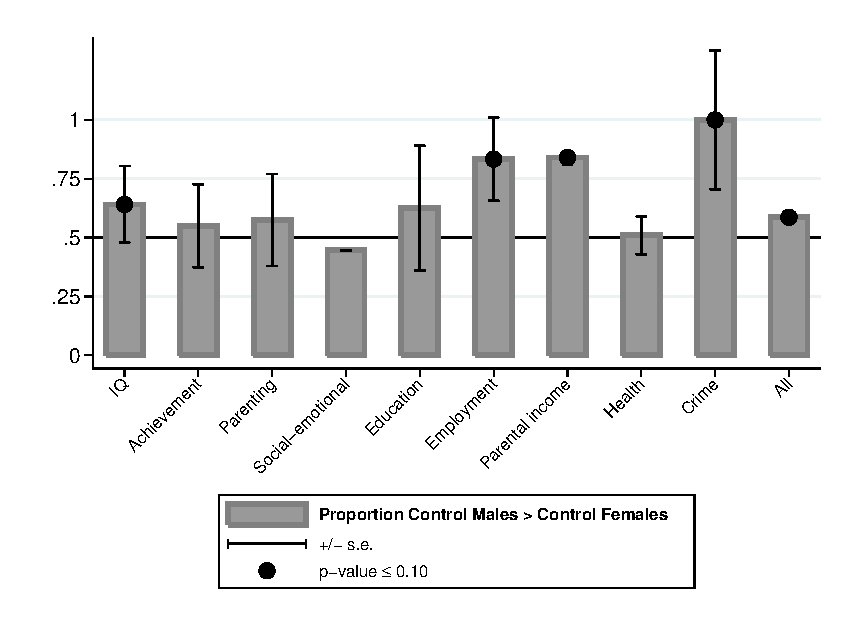
\includegraphics[width=\textwidth]{output/gendergaps-fullcontrol}
\end{sidewaysfigure}

\begin{sidewaysfigure}[H]
\centering
\caption{Proportion of Outcomes Males $>$ Females, Treatment Group}\label{fig2}
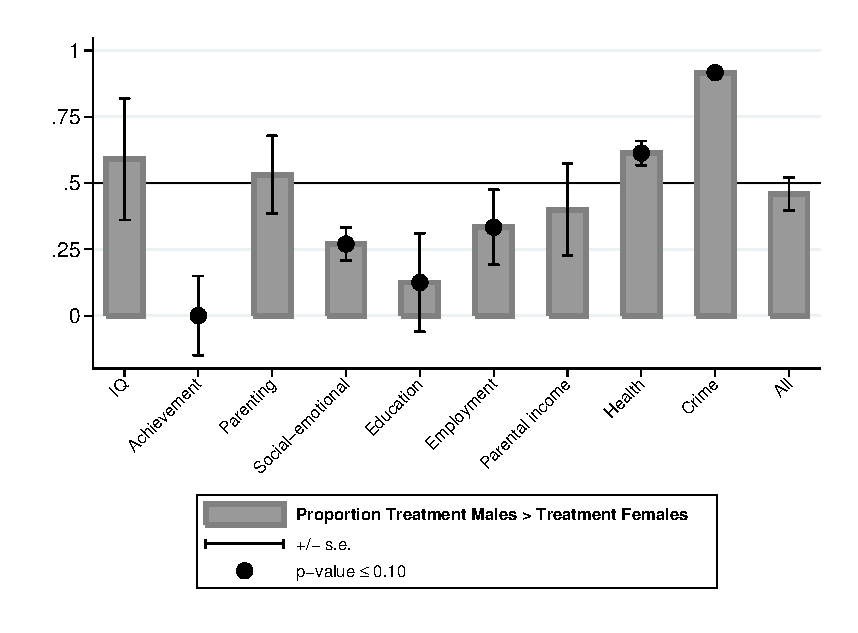
\includegraphics[width=\textwidth]{output/gendergaps-treatment}
\end{sidewaysfigure}

\begin{sidewaysfigure}[H]
\centering
\caption{Proportion of Outcomes Males $>$ Females, Control Group Divided by Alternative Setting}\label{fig3}
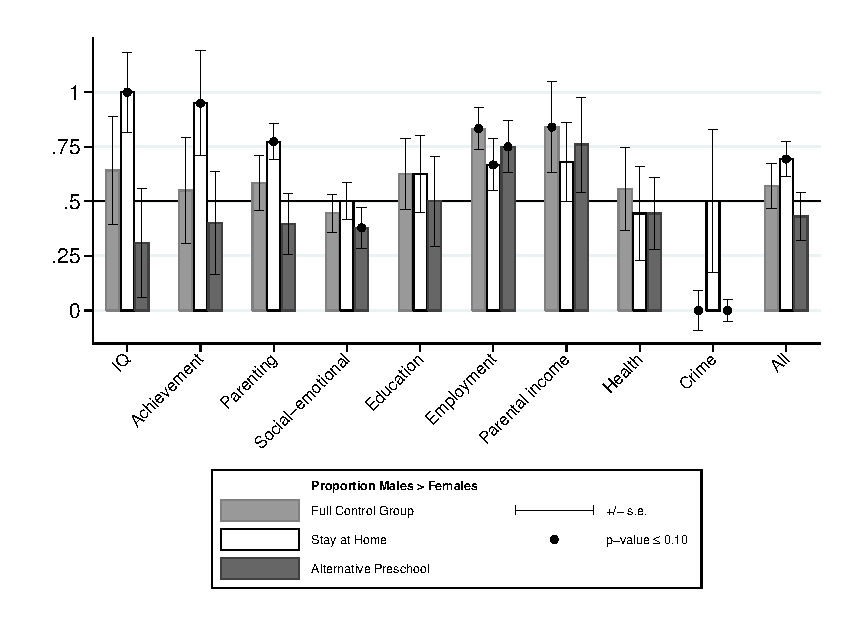
\includegraphics[width=\textwidth]{output/gendergaps-control-moderated-altpre}
\end{sidewaysfigure}

The following plots show the proportion value-added of the treatment. Let $Y_j$ be the $j$ outcome in category $J$. Then, we calculate:

\begin{equation}
	\delta = \frac{\big(\mathbb{E}[Y_j|Male, T] -\mathbb{E}[Y_j|Female, T] \big) - \big(\mathbb{E}[Y_j|Male, C] -\mathbb{E}[Y_j|Female, C] \big)}{\mathbb{E}[Y_j|Male, C] -\mathbb{E}[Y_j|Female, C]}
\end{equation}

\noindent where $T$ is treatment and $C$ is control. We then calculate the following proportion for some outcome category $J$.

\begin{equation}
	\frac{1}{|J|}\sum_j 1 \big( \delta > 0 \big).
\end{equation}

When $\delta > 0$, that means that male-female gap widens with treatment. If $\delta >0$ is present for more variables in an outcome category, than the male-female gap is widening for more of the variables. Note that for health variables, there are several variables for which the treatment has a negative effect on females. 

Figure~\ref{fig4} considers the full control group. Figure~\ref{fig5} considers those in the control group who stayed at home. Figure~\ref{fig6} considers those in the control group who attended preschool alternatives.

\begin{sidewaysfigure}[H]
\centering
\caption{Proportion of Value-added Proportions $>$ 0, Full Control Group}\label{fig4}
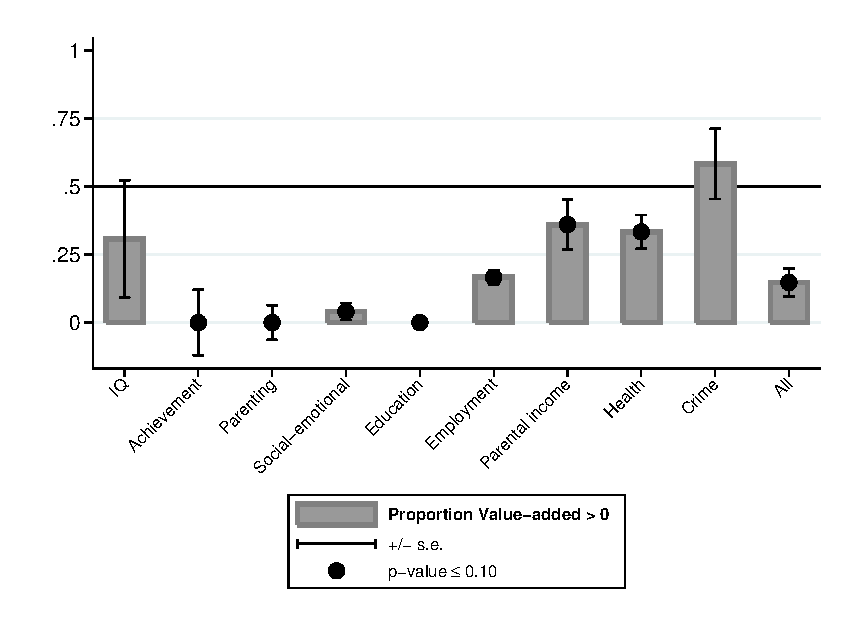
\includegraphics[width=\textwidth]{output/gendergaps-valueadded-proportion}
\end{sidewaysfigure}

\begin{sidewaysfigure}[H]
\centering
\caption{Proportion of Value-added Proportions $>$ 0, Relative to Staying at Home}\label{fig5}
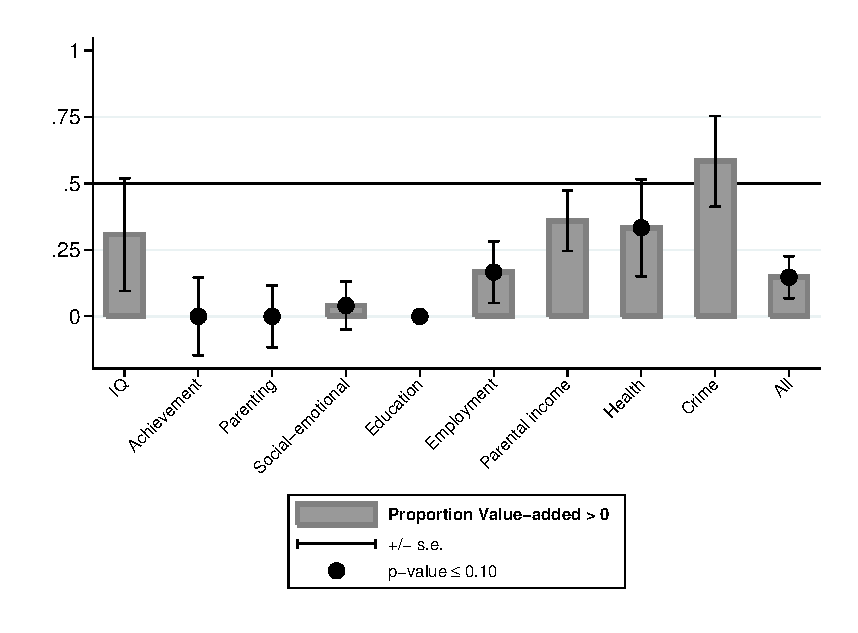
\includegraphics[width=\textwidth]{output/gendergaps-valueadded-proportion-home}
\end{sidewaysfigure}

\begin{sidewaysfigure}[H]
\centering
\caption{Proportion of Value-added Proportions $>$ 0, Relative to Alternative Preschool}\label{fig6}
\includegraphics[width=\textwidth]{output/gendergaps-valueadded-proportion-alt}
\end{sidewaysfigure}

%\begin{sidewaysfigure}[H]
%\centering
%\caption{Proportion of Outcomes Males $>$ Females, Control Group Divided by Father Present}
%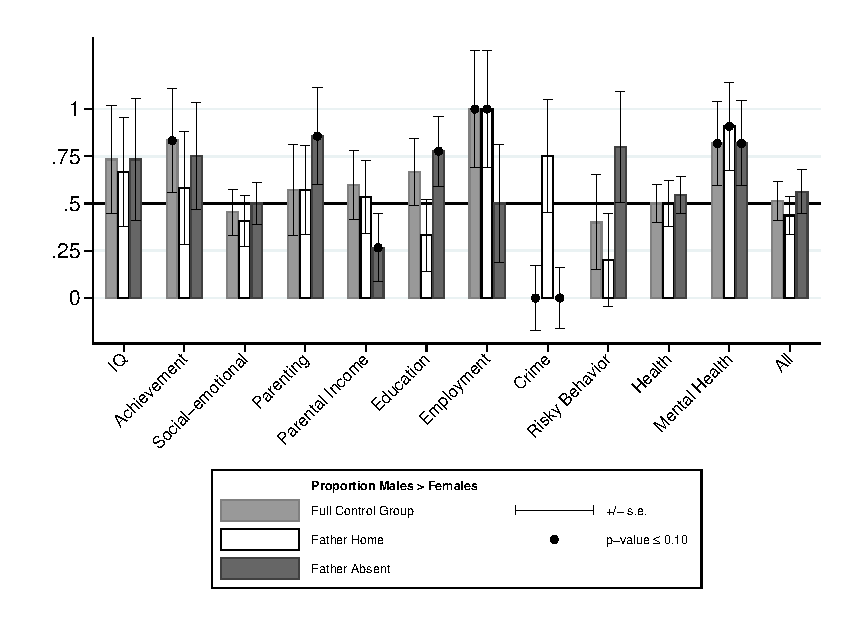
\includegraphics[width=\textwidth]{output/gendergaps-control-moderated-fhome}
%\end{sidewaysfigure}
%
%\begin{sidewaysfigure}[H]
%\centering
%\caption{Proportion of Outcomes Males $>$ Females, Treatment Group Divided by Father Present}
%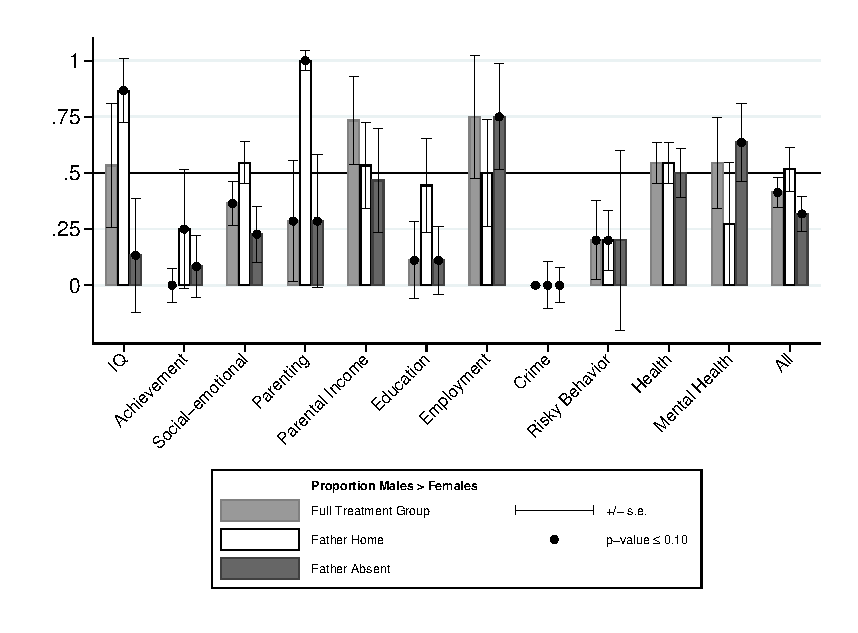
\includegraphics[width=\textwidth]{output/gendergaps-treatment-moderated-fhome}
%\end{sidewaysfigure}
%
%\begin{sidewaysfigure}[H]
%\centering
%\caption{Proportion of Outcomes Males $>$ Females, Control Group Divided by Father Present and Alternative Setting}
%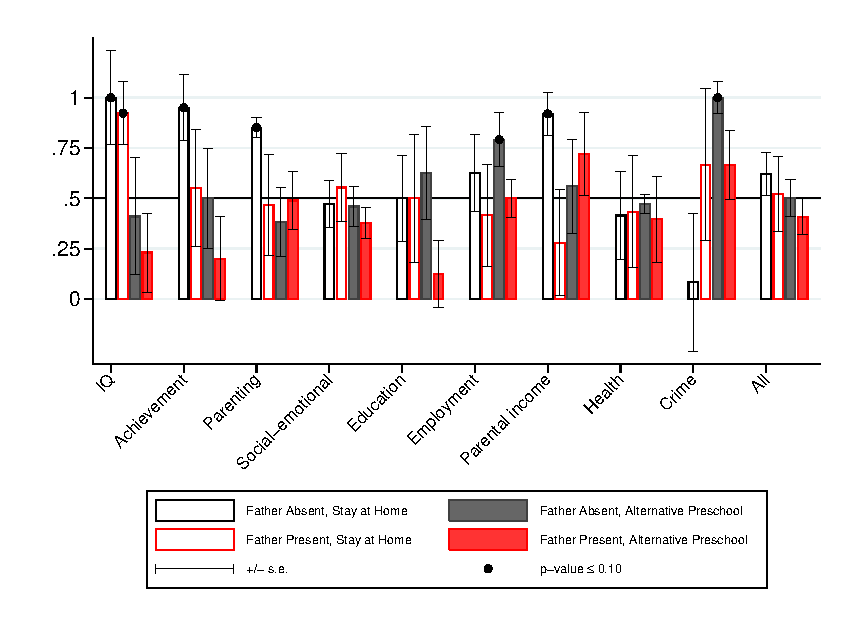
\includegraphics[width=\textwidth]{output/gendergaps-control-moderated-altpre-fhome}
%\end{sidewaysfigure}


\end{document}